% Arch 4B --- Frozen CLIP + private bottleneck adapters (M15b)
% Compile: tectonic arch4b_frozen_bottleneck.tex
\documentclass[11pt]{article}
\usepackage[a4paper,landscape,margin=14mm]{geometry}
\usepackage{lmodern}
\usepackage{amsmath,amssymb}
\usepackage{xcolor}
\usepackage{array,booktabs}
\usepackage{tikz}
\usetikzlibrary{arrows.meta,positioning,fit,backgrounds,calc}
\pagestyle{empty}
\setlength{\parindent}{0pt}
\newcolumntype{L}[1]{>{\raggedright\arraybackslash}p{#1}}

\definecolor{box}{HTML}{EEF2F7}
\definecolor{trn}{HTML}{FCE9C8}
\definecolor{frz}{HTML}{DCE6F2}
\definecolor{prv}{HTML}{E3F1DF}
\definecolor{nov}{HTML}{F8E6EF}

\tikzset{
  blk/.style={draw,rounded corners=3pt,fill=box,align=center,font=\normalsize,minimum height=18mm,text width=46mm,line width=0.8pt},
  frz/.style={blk,fill=frz},
  trn/.style={blk,fill=trn},
  prv/.style={blk,fill=prv},
  nov/.style={blk,fill=nov},
  lab/.style={font=\footnotesize,text=black!80,inner sep=1.5pt},
  ar/.style={-{Latex[length=3mm]},line width=1.1pt}}

\begin{document}

\begin{center}
{\Large\bfseries Arch 4B --- Frozen Encoder + Private Bottleneck (M15b)}\\[2pt]
{\small Strongest reading of aim~1: \textbf{no} LayerNorm tuning and \textbf{no} linear $1024{\to}2$ head. Entire CLIP ViT-L/14 is frozen.}
\end{center}
\vspace{3mm}

\begin{center}
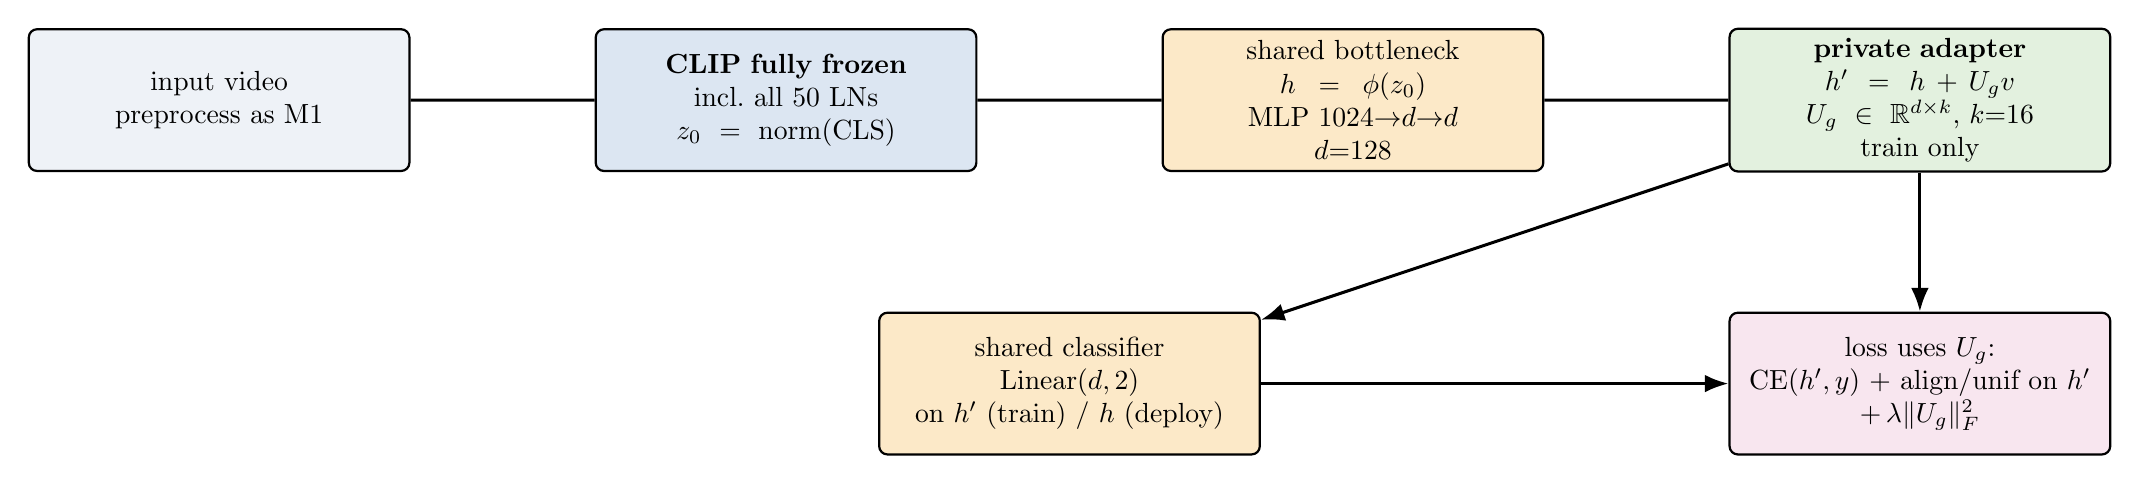
\begin{tikzpicture}[x=72mm,y=-36mm]
\node[blk] (vid) at (0,0) {input video\\preprocess as M1};
\node[frz] (enc) at (1,0) {\textbf{CLIP fully frozen}\\incl.\ all 50 LNs\\$z_0=\mathrm{norm}(\mathrm{CLS})$};
\node[trn] (bot) at (2,0) {shared bottleneck\\$h=\phi(z_0)$\\MLP $1024{\to}d{\to}d$\\$d{=}128$};
\node[prv] (ug) at (3,0) {\textbf{private adapter}\\$h'=h+U_g v$\\$U_g\in\mathbb{R}^{d\times k}$, $k{=}16$\\train only};
\node[trn] (hd) at (1.5,1) {shared classifier\\$\mathrm{Linear}(d,2)$\\on $h'$ (train) / $h$ (deploy)};
\node[nov] (loss) at (3,1) {loss uses $U_g$:\\CE$(h',y)$ + align/unif on $h'$\\$+\,\lambda\|U_g\|_F^2$};
\draw[ar] (vid)--(enc)--(bot)--(ug)--(hd);
\draw[ar] (ug)--(loss); \draw[ar] (hd)--(loss);
\end{tikzpicture}
\end{center}

\vspace{5mm}
\begin{center}
{\normalsize\bfseries Train vs deploy}
\end{center}
\vspace{2mm}
\begin{center}
\small
\begin{tabular}{L{40mm}L{70mm}L{70mm}}
\toprule
 & training (gen $g$) & inference \\
\midrule
encoder & frozen & frozen \\
bottleneck $\phi$ & trained & trained \\
private $U_g$ & active; in CE + $\lambda\|U\|_F^2$ & \textbf{discarded} ($h'=h$) \\
classifier & on $h'$ & on $h$ \\
\bottomrule
\end{tabular}
\end{center}

\vspace{6mm}
\begin{center}
\small
\begin{tabular}{L{60mm}rr}
\toprule
piece (defaults $d{=}128$, $k{=}16$) & count & deployed? \\
\midrule
shared MLP $1024{\to}128{\to}128$ & $\approx$148k$^*$ & yes \\
shared head $128{\to}2$ & 258 & yes \\
private $U_g$ ($G{\times}128{\times}16$) & 8{,}192 & no \\
LayerNorms / linear CLIP head & 0 & --- \\
\bottomrule
\end{tabular}
\end{center}
{\small $^*$If aim~4 is strict ($\lt104{,}450$), use a thinner bottleneck: e.g.\ $1024{\to}64$ only ($\approx65$k) or LoRA-style low-rank map so \textbf{deployed $\lt104{,}450$}. M15b defaults to a slim map: $z\mapsto W_2\sigma(W_1 z)$ with $W_1\in\mathbb{R}^{64\times1024}$, $W_2\in\mathbb{R}^{64\times64}$, head $64{\to}2$ $\Rightarrow$ deployed $\approx70$k still under the cap, or further reduce width to 32.}

\vspace{4mm}
\begin{center}
\small
\begin{tabular}{L{55mm}L{120mm}}
\toprule
four aims & how 4B meets them \\
\midrule
1. Not LN + linear & CLIP frozen; new bottleneck + small head \\
2. New loss & CE on adapted features + align/unif + $\lambda\|U_g\|_F^2$ \\
3. Private $\leftrightarrow$ loss & $U_g$ changes $h'$ inside CE; penalty on $U_g$ \\
4. $P\lt104{,}450$ & yes (slim bottleneck); extreme compression possible \\
\bottomrule
\end{tabular}
\end{center}

\vfill
{\small Notebook: \texttt{M15b.ipynb}. Highest risk on absolute AUC (no LN tune). Decision same gate: NT $\ge81.21$, DFD $\ge95.5$. Distinct from Arch~1/2/3: private adapters in a \textbf{learned bottleneck}, not LN/feature-centroid space.}

\end{document}
